\documentclass[14pt,a4paper]{extarticle}
\usepackage[T2A]{fontenc}
\usepackage[utf8]{inputenc}
\usepackage[english,russian]{babel}
\usepackage{lmodern}
\usepackage{geometry}
\usepackage{array}
\usepackage{tabularx}
\usepackage{longtable}
\usepackage{ltablex}
\usepackage{booktabs}
\usepackage{hyperref}
\usepackage{indentfirst}
\usepackage{microtype}
\usepackage{graphicx}
\usepackage{setspace}
\usepackage{listings}
\usepackage{graphicx}
\usepackage{caption}
\usepackage{float}
\usepackage{tocloft}
\usepackage{titlesec}
\usepackage{newtxtext,newtxmath}

\titleformat{\section}        % форматируем \section
  {\normalfont\bfseries}      % стиль: обычный + жирный
  {\thesection.}              % номер секции с точкой
  {2mm}                       % расстояние между номером и текстом
  {}                           % перед заголовком можно добавить что-то
\titlespacing*{\section}{1.5cm}{*3}{*1}  % {отступ слева}{отступ сверху}{отступ снизу}

\captionsetup{justification=centering}
\renewcommand{\ttdefault}{cmtt}
\keepXColumns
\setlength{\parindent}{3em}
\newgeometry{left=2.5cm,right=2.5cm,top=3cm,bottom=2.5cm}

\renewcommand{\contentsname}{\hspace*{4em}{\smallСодержание}}
\setlength{\cftbeforesecskip}{0.5em}
\renewcommand{\cftsecleader}{\cftdotfill{\cftdotsep}}
\renewcommand{\cftsecaftersnum}{.\hspace{2mm}}

\title{Отчёт по дисциплине "Системная инженерия"}
\author{Выполнил студент группы М-РИТ-25-1, Станиславчук Сергей}

\begin{document}

\setstretch{1.5}
\noindent
\begin{minipage}[t]{0.01\textwidth}
    \includegraphics{~/programmer/++Programmer/5_1/LSTU.jpg}
\end{minipage}%
\begin{minipage}[c]{1.1\linewidth}
    \centering
    {\small
    МИНИСТЕРСТВО НАУКИ И ВЫСШЕГО ОБРАЗОВАНИЯ РФ \\[1em]
    ФЕДЕРАЛЬНОЕ ГОСУДАРСТВЕННОЕ БЮДЖЕТНОЕ \\
    ОБРАЗОВАТЕЛЬНОЕ УЧРЕЖДЕНИЕ ВЫСШЕГО ОБРАЗОВАНИЯ \\
    «ЛИПЕЦКИЙ ГОСУДАРСТВЕННЫЙ ТЕХНИЧЕСКИЙ УНИВЕРСИТЕТ»
    }
\end{minipage}%

\vspace{3em}

\noindent
\hspace{1em}%
\begin{minipage}[t]{0.8\textwidth}
\textbf{Институт} \hspace{2em} компьютерных наук \\
\textbf{Кафедра} \hspace{2em} автоматизированных систем управления
\end{minipage}


\vspace{6em}

\begin{center}
\textbf{Индивидуальное домашнее задание №2} \\
по дисциплине \\ <<Системная инженерия>>
\end{center}

\vspace{6em}

\noindent
\begin{tabular*}{\textwidth}{@{\extracolsep{\fill}} l c r }
    Студент М-РИТ-25-1 & \makebox[4cm]{\hrulefill} & Станиславчук С.М. \\[2em]
Руководитель & \\
Профессор, канд. тех. наук & \makebox[4cm]{\hrulefill} & Качановский Ю.П. \\
\end{tabular*}

\vfill
\begin{center}
    Липецк, 2026
\end{center}

\thispagestyle{empty}

\newpage
\tableofcontents
\newpage

\section{Задание кафедры}
\begin{sloppypar}
    Перевести и выступить с презентацией содержания базовых нормативных документов системной инженерии
    Мой вариант: 2.13.
    Part 3. Systems Engineering and Management
    Part 3c: Processes c. 607-640
    Knowledge Area: System Maintenance
\end{sloppypar}

\section{Область знаний: Сопровождение систем (System Maintenance)}

\subsection{Содержание данной области знаний}

\begin{itemize}
\item Логистика (Scott Jackson и John Snoderly) (Garry Roedler)
\item Управление жизненным циклом эксплуатации (William Stiffler)
\item Продление жизненного цикла эксплуатации (William Stiffler) (Brian Wells)
\item Обновления возможностей, модернизация и улучшения (William Stiffler) (Brian Wells)
\item Вывод системы из эксплуатации и утилизация (Brian Wells)
\item Ведущие авторы:
    \begin{itemize}
        \item Scott Jackson и Brian Gallagher
    \end{itemize}
\item Участвующий автор:
    \begin{itemize}
        \item David Dorgan
    \end{itemize}
\end{itemize}

\hrule

Планирование сопровождения системы начинается на ранних этапах процесса приобретения с разработки концепции сопровождения. Планирование проводится для формирования и уточнения требований и задач, необходимых для достижения, восстановления и поддержания эксплуатационной готовности системы на протяжении всего жизненного цикла. Чтобы система могла поддерживаться в течение всего жизненного цикла, процесс сопровождения должен выполняться параллельно с процессом эксплуатации (ISO/IEC/IEEE 15288:2015, пункт 6.4.9).

\hrule

\section{Темы}

Каждая часть SEBoK делится на области знаний (KA), которые представляют собой группы информации, объединённые общей тематикой. Эти области, в свою очередь, делятся на темы. Данная область включает:

\begin{itemize}
\item Логистика
\item Управление жизненным циклом эксплуатации
\item Продление жизненного цикла эксплуатации
\item Обновления возможностей, модернизация
\item Вывод из эксплуатации и утилизация
\end{itemize}

\section{Обзор}

Начальные требования к сопровождению должны быть определены на этапе формирования потребностей заинтересованных сторон (пункт 6.4.1 ISO/IEC/IEEE 15288:2015) и продолжают развиваться в ходе разработки и эксплуатации системы. Ключевые аспекты:

\begin{itemize}
\item Максимизация доступности системы для выполнения эксплуатационных требований с учётом заложенной надёжности и ремонтопригодности, а также доступных ресурсов
\item Сохранение эксплуатационного потенциала за счёт корректного планирования обслуживания, включая стратегию обслуживания, ориентированную на надёжность, с внедрением профилактического обслуживания для предотвращения отказов и увеличения среднего времени между ремонтами
\end{itemize}

Дополнительно:

\begin{itemize}
\item Разделение задач обслуживания с возможностью передачи некритичных работ подрядчикам
\item Использование ИТ-технологий для управления обслуживанием (сбор и анализ данных эксплуатации и обслуживания)
\end{itemize}

Управление обслуживанием включает разработку и пересмотр планов обслуживания, а также обеспечение и координацию ресурсов (бюджет, запчасти, поддерживающие процессы и т.д.). Планирование обслуживания опирается на анализ уровня ремонта (LORA) в рамках процесса приобретения. Начальное планирование направлено на минимизацию стоимости жизненного цикла (LCC).

\section{Подходы к процессу}

Цель процесса сопровождения — поддержание способности системы предоставлять услуги. Процесс:

\begin{itemize}
\item контролирует способность системы выполнять функции
\item выявляет проблемы
\item реализует корректирующие, адаптивные, предупредительные действия
\item подтверждает восстановление работоспособности
\end{itemize}

Результаты эффективного сопровождения:

\begin{itemize}
\item разработана стратегия обслуживания
\item ограничения обслуживания учтены в требованиях
\item обеспечена доступность заменяемых элементов
\item поддерживается соответствие услуг требованиям заинтересованных сторон
\item выявляется необходимость изменений конструкции
\item ведётся учёт данных об отказах
\end{itemize}

Проект должен реализовывать следующие виды деятельности:

\begin{itemize}
\item плановое обслуживание (осмотры, сервис, очистка)
\item внеплановое обслуживание (диагностика, локализация и замена неисправных элементов)
\item перенастройка системы под различные функции
\item более сложное плановое обслуживание (ниже уровня капитального ремонта)
\item сложное внеплановое обслуживание
\item незначительные модификации
\item мелкий ремонт
\item капитальное обслуживание (например, капитальный ремонт, антикоррозийная обработка)
\item крупный ремонт
\end{itemize}

План обслуживания определяет:

\begin{itemize}
\item плановые работы (профилактика)
\item внеплановые работы (адаптивные и корректирующие)
\item распределение задач между организациями
\end{itemize}

Также формируется распределение задач по исполнителям: внутренние подразделения, подрядчики, OEM и т.д., а также требования к ресурсам поддержки.

Связанные активности:

\begin{itemize}
\item планирование ресурсов
\item бюджетирование
\item мониторинг эффективности
\item модернизация
\item долгосрочная поддержка
\item устойчивость
\end{itemize}

Все они выполняются на протяжении всего жизненного цикла системы.

\section{Обучение и сертификация}

Технический персонал должен проходить соответствующее обучение. Помимо начального обучения, требуется дополнительная подготовка:

\begin{itemize}
\item при увеличении количества систем
\item при текучести кадров
\item при модернизации системы
\end{itemize}

Необходимо заранее определить стандарты сертификации и включить требования к обучающим материалам в контракт поставки.

\section{Практические соображения}

Организация должна определить чёткие критерии, когда:

\begin{itemize}
\item изменение можно выполнить в рамках сопровождения
\item требуется полноценный проект с прохождением полного жизненного цикла разработки
\end{itemize}

Критерии включают:

\begin{itemize}
\item стоимость
\item сроки
\item риски
\item критичность
\end{itemize}

\hrule


\subsection{Определение логистики}

\textbf{Дополнительные ссылки}

Отсутствуют.

\textbf{Логистика}

\begin{itemize}
\item \textbf{Ведущие авторы:} Скотт Джексон и Джон Сноддерли
\item \textbf{Соавтор:} Гарри Рёдлер
\end{itemize}

Существует несколько определений логистики в рамках системной инженерии (SE), и используемое определение устанавливает, какие виды деятельности считаются частью логистики. \textbf{SEBoK} определяет логистику как науку планирования и реализации приобретения и использования ресурсов, необходимых для поддержания функционирования системы.

\subsubsection{Обзор}

Способность поддерживать функционирование системы определяется внутренней поддерживаемостью системы (функцией проектирования) и процессами, используемыми для поддержания функций и возможностей системы в контексте конечного пользователя. На рисунке 1 ниже показана модель Академии закупок Министерства обороны США (DAU), отражающая аспекты системной инженерии, которые следует учитывать в логистике и логистическом планировании (DAU 2010).

\begin{figure}[H]
    \label{fig:1}
    \centering
    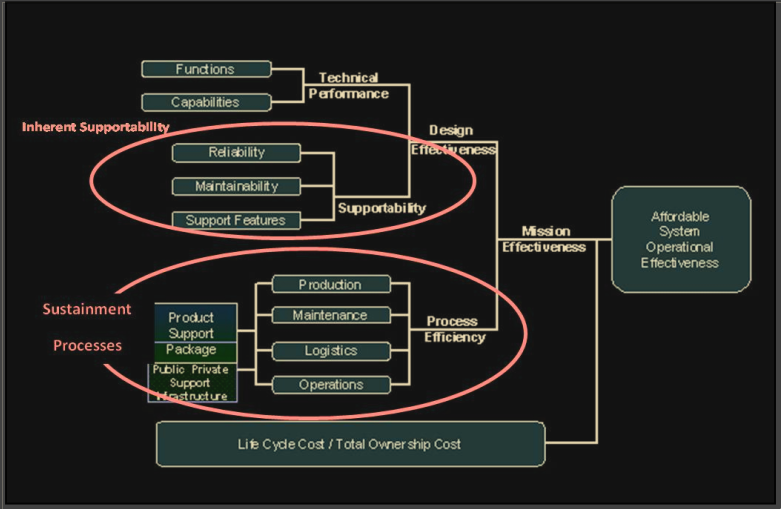
\includegraphics[width=0.78\textwidth]{fig1.png}
    \refstepcounter{figure}
    \caption*{Рисунок \thefigure\ — Доступная оперативная эффективность системы (Руководство DAU 2010)}
\end{figure}
\textit{Опубликовано Академией закупок Министерства обороны США (DAU)/Министерством обороны США (DoD).}

\hrule

\subsection{Планирование поддержки}

Основное внимание при планировании поддержки уделяется влиянию на внутреннюю поддерживаемость системы, а также планированию возможностей и процессов, которые будут использоваться для поддержания функционирования системы.

\subsubsection{Влияние на внутреннюю поддерживаемость (Эксплуатационная пригодность)}

Влияние на поддержку требует понимания концепции эксплуатации (ConOps), миссий системы, профилей миссий и системных возможностей для понимания обоснования функциональных приоритетов и приоритетов производительности. Понимание обоснования открывает путь к принятию решений о необходимых компромиссах между производительностью системы, доступностью и стоимостью жизненного цикла (LCC), что влияет на экономическую эффективность эксплуатации, технического обслуживания и логистической поддержки системы.

Не существует единого списка факторов поддержки или конкретного способа их группировки, поскольку они тесно взаимосвязаны. Они включают: совместимость, интероперабельность, транспортабельность, надежность, ремонтопригодность, потребность в персонале, человеческие факторы, безопасность, воздействие природной среды, диагностику и прогнозирование, а также защиту от коррозии и её смягчение.

Ниже приведены ключевые проектные соображения:

\begin{itemize}
\item \textbf{Архитектурные соображения} — фокус на открытости, модульности, масштабируемости и модернизации. Требуются компромиссы между атрибутами.
\item \textbf{Соображения надежности} — определяют эффективность системы и логистическую нагрузку. Цель — минимизация риска отказа при заданных ограничениях.
\item \textbf{Соображения ремонтопригодности} — снижение затрат и времени обслуживания. Ремонтопригодность должна быть встроенной.
    \begin{itemize}
    \item \textbf{Модульность} — замена компонентов вместо ремонта.
    \item \textbf{Интероперабельность} — использование стандартных интерфейсов.
    \end{itemize}
\end{itemize}

\subsubsection{Продолжение планирования поддержки}

\begin{itemize}
\item \textbf{Физическая доступность} — доступ к обслуживаемым компонентам
\item \textbf{Минимизация профилактического обслуживания}
\item \textbf{Встроенное обучение и тестирование}
\item \textbf{Интеграция человеческих систем (HSI)}
\item \textbf{Соображения поддержки} — должны учитываться на этапе проектирования
\end{itemize}

\subsection{Компоненты логистики}

\textbf{Логистика}

\begin{itemize}
\item Управление рисками
\item \textbf{Интерфейс проектирования}
    \begin{itemize}
    \item надежность
    \item ремонтопригодность
    \item поддерживаемость
    \item доступность
    \item управление конфигурацией
    \item безопасность
    \item экологические требования
    \item HSI
    \item калибровка
    \item anti-tamper
    \item обитаемость
    \item утилизация
    \item правовые требования
    \end{itemize}
\item \textbf{Инжиниринг поддержки}
    \begin{itemize}
    \item FRACAS
    \item Value engineering
    \item DMSMS
    \end{itemize}
\item Материально-техническое снабжение
\item Планирование технического обслуживания
\item Вспомогательное оборудование
\item Техническая документация
\item Персонал
\item Обучение
\item Инфраструктура
\item Упаковка и транспортировка
\item Вычислительные ресурсы
\end{itemize}

\subsection{Реализация поддержки}

После ввода системы в эксплуатацию начинается реализация поддержки. Системная инженерия обеспечивает выполнение элементов комплексной поддержки продукта (IPS) для достижения эксплуатационных требований с минимальной стоимостью жизненного цикла.

\subsubsection{Элементы IPS}

\begin{enumerate}
\item Управление поддержкой продукта
\item Интерфейс проектирования
\item Инжиниринг поддержки
\item Планирование обслуживания
\item Материально-техническое снабжение
\item Упаковка и транспортировка
\item Вспомогательное оборудование
\item Техническая документация
\item Персонал
\item Обучение
\item Инфраструктура
\item Вычислительные ресурсы
\end{enumerate}

\subsubsection{Процесс системной инженерии}

\textbf{Управление}
\begin{itemize}
\item Техническое планирование
\item Управление рисками
\item Оценка усилий
\item Контроль базовой линии
\end{itemize}

\textbf{Техническая часть}
\begin{itemize}
\item Разработка требований
\item Архитектура системы
\item Анализ и оптимизация
\item Верификация и валидация
\end{itemize}

\textbf{Инфраструктура}
\begin{itemize}
\item Процессы
\item Инструменты
\item Обучение
\item Оценка возможностей
\item Управление технологиями
\end{itemize}

\subsubsection{Входные и выходные данные}

\textbf{Входные данные}
\begin{itemize}
\item Планы программы
\item Базовые линии системы
\item Техническое задание
\end{itemize}

\textbf{Выходные данные}
\begin{itemize}
\item Обновленные планы
\item Обновленная система
\end{itemize}

\subsubsection{Деятельность SE}

\begin{enumerate}
\item Сбор данных эксплуатации
\item Анализ причин проблем
\item Оценка рисков
\item Разработка корректирующих действий
\item Тестирование
\item Оценка улучшений
\item Внедрение
\end{enumerate}


\begin{figure}[H]
    \label{fig:2}
    \centering
    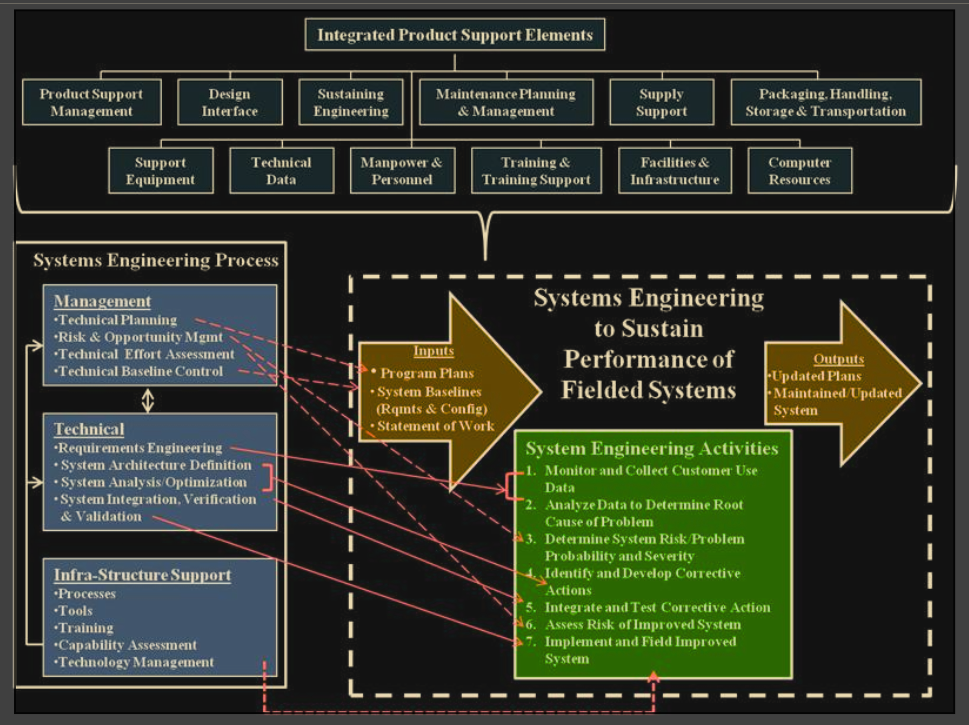
\includegraphics[width=0.78\textwidth]{fig2.png}
    \refstepcounter{figure}
    \caption*{Рисунок \thefigure\ — Реализация поддержки (DAU 2012)}
\end{figure}

После ввода системы в эксплуатацию SE используется для исправления проблем и улучшения системы. Изменения должны учитывать все элементы IPS и их взаимосвязи.

Степень изменений варьируется от незначительных корректировок до полного перепроектирования системы.

Эволюционные системы требуют подхода «система систем» (SoS) для синхронизации основной системы и поддержки.


\subsection{Управление жизненным циклом продукции и услуг}

Область знаний, связанная с управлением жизненным циклом продукции и услуг, включает следующие области:

\begin{enumerate}
\item \textbf{Продление срока службы (Service Life Extension)} — системным инженерам необходимо понимать принципы продления срока службы, проблемы модификации систем, а также вопросы утилизации и вывода из эксплуатации.

\item \textbf{Модернизация и обновления (Modernization and Upgrades)} — управление продлением срока службы использует процессы управления инженерными изменениями с учётом ограничений срока службы. Модернизация устаревших систем требует полного понимания интерфейсов и технической документации.

\item \textbf{Утилизация и вывод из эксплуатации (Disposal and Retirement)} — требует учёта экологических аспектов, обработки опасных отходов и синхронизации с вводом заменяющей системы.
\end{enumerate}

\subsubsection{Принципы и стандарты}

Принципы управления жизненным циклом применимы к различным типам систем. Тип системы (коммерческая или государственная) определяет выбор стандартов и практик.

Военные системы США опираются на материалы Министерства обороны (DoD), включая Академию закупок (DAU) и органы стандартизации, такие как AIAA, SAE, SOLE, OGC.

Коммерческие отрасли (авиация, энергетика, транспорт, водоснабжение, интернет, медицина) используют стандарты и практики государственных и коммерческих организаций, включая DOT, ISO, IEEE, INCOSE.

Некоторые организации разрабатывают универсальные подходы (INCOSE, SOLE, ISO, IEEE).

Среди коммерческих ассоциаций:

\begin{itemize}
\item ASHE
\item ACM
\item ASME
\item ASTM
\item NAHB
\item ISOC (включая IETF)
\item SAE
\end{itemize}

\subsubsection{Ресурсы}

\begin{itemize}
\item \textbf{INCOSE Systems Engineering Handbook} (v3.2.2)
\item \textbf{Systems Engineering Guidebook for ITS} (Caltrans, USDOT)
\item \textbf{Systems Engineering and Analysis} (Blanchard, Fabrycky)
\item \textbf{Modernizing Legacy Systems} (Seacord et al.)
\item \textbf{Logistics and Materiel Readiness} (OUSD)
\end{itemize}

\hrule

\subsection{Хорошие практики и заключение}

\textbf{Хорошие практики (Good Practices)}

Основных проблем можно избежать, если системный инженер:

\begin{itemize}
\item признаёт, что системная инженерия продолжается после ввода системы в эксплуатацию
\item понимает роль функций управления жизненным циклом
\item обеспечивает соответствие модификаций требованиям
\item учитывает непрерывность процессов обслуживания
\item принимает во внимание изменяющиеся требования пользователей
\item адаптирует концепции поддержки
\item применяет управление инженерными изменениями ко всей системе
\end{itemize}

Игнорирование этих аспектов приводит к серьёзным последствиям.

\subsection*{Ссылки}

\textbf{Цитируемые работы}

\begin{itemize}
\item Blanchard, B.S. and W.J. Fabrycky. 2011. \textit{Systems Engineering and Analysis}, 5th ed.
\item Caltrans and USDOT. 2005. \textit{Systems Engineering Guidebook for Intelligent Transportation Systems (ITS)}, version 1.1.
\item DAU. 2010. Acquisition Community Connection.
\item INCOSE. 2012. \textit{Systems Engineering Handbook}, version 3.2.2.
\item Jackson. 2007. A Multidisciplinary Framework for Resilience to Disasters and Disruptions.
\item OUSD(AT\&L). 2011. Logistics and Materiel Readiness policies.
\item Seacord, R.C., D. Plakosh, and G.A. Lewis. 2003. \textit{Modernizing Legacy Systems}.
\end{itemize}

\subsection{Управление жизненным циклом продукции и услуг (Service Life Management)}

\begin{itemize}
\item \textbf{Соавтор:} Уильям Стиффлер
\end{itemize}

\hrule

Управление жизненным циклом продукции и услуг занимается общим планированием жизненного цикла и поддержкой системы. Срок службы продукта или услуги значительно превышает время, необходимое для проектирования и разработки. Системные инженеры должны применять принципы управления жизненным циклом на всех этапах существования системы. Основное внимание уделяется изменениям после развертывания: продлению срока службы, модернизации, утилизации и выводу из эксплуатации.

\subsubsection{Обзор}

Управление жизненным циклом также называется \textit{поддержкой системы (system sustainment)}. Оно включает обеспечение поддерживаемости системы от закупки до утилизации и напрямую влияет на производительность и стоимость эксплуатации.

К мероприятиям поддержки относятся:

\begin{itemize}
\item проектирование для ремонтопригодности
\item встроенное тестирование
\item диагностика и прогностика
\item обслуживание по состоянию
\item сокращение логистического «следа»
\item внедрение новых технологий
\item снижение затрат эксплуатации
\item мониторинг показателей поддержки
\end{itemize}

Для сложных систем формируются планы поддержки жизненного цикла. Подход применим как к коммерческим, так и к государственным системам.

Критически важно учитывать поддержку уже на этапе определения требований, включая анализ стоимости жизненного цикла и стратегию сопровождения.

\hrule

\subsubsection{Области знаний}

\begin{enumerate}
\item \textbf{Продление срока службы} — включает управление модификациями и подготовку к завершению жизненного цикла.
\item \textbf{Модернизация и обновления} — требует управления инженерными изменениями и полного понимания архитектуры системы.
\item \textbf{Утилизация и вывод из эксплуатации} — учитывает экологические требования и синхронизацию с заменяющими системами.
\end{enumerate}

\subsection{Принципы и стандарты}

Подходы зависят от типа системы.

Военные системы используют стандарты DoD, DAU, AIAA, SAE, SOLE, OGC.

Коммерческие системы опираются на стандарты DOT, ISO, IEEE, INCOSE и др.

Универсальные стандарты разрабатываются организациями INCOSE, ISO, IEEE, SOLE.

Коммерческие ассоциации:

\begin{itemize}
\item ASHE
\item ACM
\item ASME
\item ASTM
\item NAHB
\item ISOC (включая IETF)
\item SAE
\end{itemize}

\subsubsection{Ресурсы}

\begin{itemize}
\item INCOSE Systems Engineering Handbook
\item ITS Systems Engineering Guidebook
\item Systems Engineering and Analysis
\item Modernizing Legacy Systems
\item Logistics and Materiel Readiness
\end{itemize}

\hrule

\subsection{Лучшие практики}

Дополнительный источник:

\begin{itemize}
\item \textit{A Multidisciplinary Framework for Resilience to Disasters and Disruptions}
\end{itemize}

\subsubsection{Good Practices}

\begin{itemize}
\item признание непрерывности системной инженерии после ввода в эксплуатацию
\item понимание роли управления жизненным циклом
\item соответствие модификаций требованиям
\item сохранение процессов обслуживания
\item учет изменения требований пользователей
\item адаптация стратегий поддержки
\item применение управления изменениями ко всей системе
\end{itemize}

Игнорирование этих факторов приводит к серьёзным последствиям.

\subsection*{Ссылки}

\subsection{Продление срока службы (Service Life Extension)}

\begin{itemize}
\item \textbf{Ведущий автор:} Уильям Стиффлер
\item \textbf{Соавтор:} Брайан Уэллс
\end{itemize}

\hrule

Продление срока службы продукта и/или услуги предполагает продолжение использования за пределами первоначального расчетного срока. Оно включает анализ рисков и стоимости жизненного цикла (LCC) по сравнению с заменой системы.

Основной акцент делается на повышении надежности, замене и восстановлении компонентов для отсрочки перехода системы в состояние износа. Цель — приблизить состояние системы к новому в рамках экономических ограничений.

СЛП также рассматривается как экологически оправданный подход, позволяющий избежать преждевременной утилизации. Ключевая проблема — определить целесообразность продления срока службы в условиях технологических изменений и физического износа.

\subsubsection{Обзор темы}

СЛП применяется, если:

\begin{itemize}
\item система не соответствует требованиям надежности или производительности
\item стоимость эксплуатации превышает допустимые пределы
\item отсутствуют запасные части
\item нарушаются нормативные требования
\item элементы достигают пределов ресурса
\end{itemize}

Предпочтителен упреждающий подход, позволяющий выполнять СЛП до критического ухудшения характеристик.

Ключевые факторы:

\begin{itemize}
\item текущая стоимость жизненного цикла
\item расчетный и остаточный срок службы
\item сопровождение ПО
\item управление конфигурацией
\item гарантийная политика
\item доступность компонентов
\item наличие документации
\end{itemize}

Расчетный срок службы определяется на этапе проектирования и зависит от ограничений безопасности и старения материалов. Системы, подверженные усталости (например, мосты, самолеты), требуют регулярной диагностики.

\subsubsection{Программное обеспечение, материалы и продукты}

Сопровождение программного обеспечения — критический аспект. Устаревшие системы часто сохраняются из-за высокой стоимости замены.

Продление срока службы может обеспечиваться за счёт выбора материалов (например, эпоксидная арматура в инфраструктуре).

Проблема DMSMS (исчезающие поставщики и компоненты) должна учитываться заранее.

При СЛП необходимо пересматривать допущения анализа LCC.

\subsubsection{Применение к продуктовым системам}

Решение о СЛП принимается на основе сравнения LCC существующей и новой системы.

Военные системы используют формализованные программы SLEP и непрерывную модернизацию.

Примеры:

\begin{itemize}
\item B-52 (с 1955 года)
\item Boeing 737 (с 1967 года)
\end{itemize}

Для критических систем (например, ядерных реакторов) приоритет — безопасность.

\subsubsection{Применение к сервисным системам}

СЛП сервисных систем требует непрерывности предоставления услуг и поэтапного внедрения изменений.

Примеры:

\begin{itemize}
\item транспортные системы
\item системы водоснабжения
\item энергетические системы
\item здравоохранение
\end{itemize}

Системы водоснабжения — пример долгоживущих систем, требующих постоянной модернизации.

\subsubsection{Применение к предприятиям}

СЛП предприятий требует системного подхода ко всем подсистемам.

Примеры:

\begin{itemize}
\item космические системы (NASA)
\item нефтегазовые системы
\end{itemize}

Продление срока службы может достигаться за счет внедрения технологий (например, повышение нефтеотдачи пластов).

\subsubsection{Другие темы}

Необходимо учитывать требования по хранению данных и нормативные ограничения.

\subsubsection{Практические соображения}

\begin{itemize}
\item сравнение стоимости СЛП и новой системы
\item распределение финансирования во времени
\item минимизация сбоев при модернизации
\item учет морального устаревания компонентов
\end{itemize}
\hrule


\subsection{Обновление возможностей, модернизация и апгрейд (Capability Updates, Upgrades, and Modernization)}

\begin{itemize}
\item \textbf{Ведущий автор:} Уильям Стиффлер
\item \textbf{Соавтор:} Брайан Уэллс
\end{itemize}

Модернизация и обновление включают изменение продукта или услуги для добавления новых функций, улучшения производительности и поддерживаемости. На определённом этапе жизненного цикла требуется модернизация для снижения эксплуатационных затрат и решения проблем поддержки. Ключевым фактором принятия решений является стоимость жизненного цикла (LCC).

Проектирование с учётом будущей модернизации должно выполняться на ранних этапах. Используются предложения по инженерным изменениям (ECP). Важным принципом является F3I (форма, соответствие, функция, интерфейс) для обеспечения обратной совместимости.

\subsubsection{Обзор темы}

Модернизация использует стандартные процессы системной инженерии, но ограничена существующей архитектурой системы.

Причины модернизации:

\begin{enumerate}
\item снижение производительности, безопасности или надёжности
\item потребность в новых функциях
\item устаревание компонентов
\item новые сценарии использования
\end{enumerate}

Модернизация устаревших систем требует глубокого понимания существующей системы и её ограничений.

\subsubsection{Ключевые факторы и процессы}

\textbf{Факторы:}

\begin{itemize}
\item тип системы
\item сценарии использования
\item правовые требования
\item LCC
\item использование спектра
\item доступность поставщиков
\item документация системы
\item интеграция и интероперабельность
\item объём регрессионного тестирования
\end{itemize}

\textbf{Процессы:}

\begin{itemize}
\item сертификация
\item анализ безопасности
\item управление изменениями
\item анализ альтернатив
\item гарантийная политика
\item управление поставками
\end{itemize}

\subsubsection{Применение к продуктовым системам}

Модернизация требует:

\begin{itemize}
\item управления изменениями (change control boards)
\item использования FMECA
\item обновления документации
\item анализа ConOps
\end{itemize}

При отсутствии документации применяется обратный инжиниринг.

Регрессионное тестирование необходимо для проверки неизменённых функций. Используется матрица прослеживаемости требований.

Также учитываются изменения в элементах поддержки системы.

Некоторые системы (например, потребительская электроника) нецелесообразно модернизировать.

\subsubsection{Применение к сервисным системам}

Требуется:

\begin{itemize}
\item соблюдение нормативных требований
\item обратная совместимость
\item поэтапное внедрение
\end{itemize}

Часто необходим обратный инжиниринг.

\subsubsection{Применение к предприятиям}

Основные проблемы:

\begin{itemize}
\item внедрение без остановки системы
\item координация изменений
\item управление архитектурой
\end{itemize}

Изменения могут быть локальными или глобальными.

\subsubsection{V-образная модель}

Модификации могут вводиться на разных уровнях V-модели:

\begin{itemize}
\item верхний уровень — системные изменения
\item средний уровень — изменения подсистем
\item нижний уровень — изменения компонентов
\end{itemize}

Изменения на низком уровне должны соответствовать принципу F3I.

\subsubsection{Практические соображения}

\begin{itemize}
\item управление множественными изменениями
\item блочный метод
\item непрерывная интеграция
\item управление релизами ПО
\end{itemize}

\subsubsection{COTS-компоненты}

Преимущества:

\begin{itemize}
\item снижение стоимости
\item улучшение функциональности
\end{itemize}

Риски:

\begin{itemize}
\item устаревание
\item изменение интерфейсов
\end{itemize}

\hrule

\subsection{Утилизация и вывод системы из эксплуатации (System Disposal and Retirement)}

\begin{itemize}
\item \textbf{Ведущий автор:} Брайан Уэллс
\end{itemize}

Утилизация и вывод из эксплуатации являются завершающим этапом жизненного цикла. Система становится экономически нецелесообразной, устаревшей или неремонтопригодной.

Современная системная инженерия учитывает переработку, повторное использование и экологические требования.

\subsubsection{Обзор темы}

Цель — удалить систему из эксплуатации и безопасно обработать материалы.

Ключевые экологические факторы:

\begin{itemize}
\item загрязнение воздуха
\item загрязнение воды
\item шум
\item радиация
\item отходы
\end{itemize}

Утилизация регулируется государственными органами (например, EPA, OSHA).

\subsubsection{Применение к продуктовым системам}

Включает:

\begin{itemize}
\item утилизацию или консервацию
\item планирование удаления компонентов
\item управление опасными материалами
\item логистику и затраты
\end{itemize}

Утилизация должна планироваться заранее.

Система обращения с отходами известна как «cradle-to-grave».

\subsubsection{Практические аспекты}

\begin{itemize}
\item утилизация — наименее предпочтительный вариант
\item отсутствие прямой экономической выгоды
\item часто выполняется внешними организациями
\end{itemize}

Регуляции:

\begin{itemize}
\item RCRA
\item REACH
\item RoHS
\end{itemize}

Необходимо учитывать ограничения на материалы и требования цепочки поставок.

Вывод из эксплуатации требует детального планирования и обновления поддерживающей инфраструктуры.


\section{Вывод}
В ходе выполненного индивидуального домашнего задания изучил методы обслуживания систем программного обеспечения.

\end{document}
